% Clear the page
\clearpage
% Chaper title
\chapter{Introduction}
% Label for chapter
\label{ch1_introduction}
% Set the font size in this chapter
\normalsize
%===============================================================================
% Start of Chapter
%===============================================================================

%===============================================================================



\section{Credit for this template}
    \label{ch1_section_installation}


%===============================================================================

This template was not created by me (Neil Cook) though I added some functionality, commands and a lot of the comments, including this ``readme''. This template was passed on to me by Dr. Federico Marocco and was originally created by Dr. Kieran Forde (2007) and in various forms have been used by many of the astrophysics PhD students at the University of Hertfordshire.

%------------------------------------------------------------------------------------------------
\subsection{File structure and contents}
    \label{ch1_section_file_structure}
%------------------------------------------------------------------------------------------------

The following should be found within the extracted directory.

\begin{lstlisting}[style=base]
    ./appendices/
        appendixA.tex       
        appendixB.tex
    ./chapters/
        ch_1.tex
        ch_2.tex
    ./figures/
        phd_comics_example.jpg
        phd_comics_example1.jpg
    ./footers/
        1.jpg
        2.jpg
        ...
        225.jpg
    ./latex_resources/
        /comment/    @package from CTAN.org@
        /glossary/   @package from CTAN.org@
        /mfirstuc/   @package from CTAN.org@
        /sidecap/    @package from CTAN.org@
        /tocloft/    @package from CTAN.org@
        makeindex
    ./preamble/
        Abstract.tex 
        acknowledgement_refs.tex 
        Acknowledgements.tex
        glossary.tex 
        newcommands.tex
        symbols.tex
        titlepage.tex
    ./referencing/
        article_names.tex
        astroads.bst
        Bibliography.bib 
    ./tables/
        ch1_table_example1.tex
        ch1_table_example2.tex
        ch1_table_example_landscape.tex
    compile
    main.pdf
    main.tex
    phd.cls
\end{lstlisting}


%===============================================================================



\section{Installation and running code}
    \label{ch1_section_installation}


%===============================================================================

%------------------------------------------------------------------------------------------------
\subsection{The compiler}
    \label{ch1_section_installation_modifying_tex_path}
%------------------------------------------------------------------------------------------------

    You will not be able to just run ``pdflatex'' or ``latex'' to compile this \LaTeX document, thus you will need to run the ``compile'' file (\url{./compile}).

    The compile file runs the following set of programs (defined below) in this specific order:

    \begin{lstlisting}[style=base]
    $LATEX "$rootPath"

    $BIBTEX "$rootPath"

    $MKGLOS "$rootPath"

    $MKINDX "$rootPath"".idx"

    $MKINDX -s "$rootPath"".ist" -t "$rootPath"".glg" 
               "$rootPath"".glo" -o "$rootPath"".gls"

    $MKINDX -s "$rootPath"".ist" -t "$rootPath"".nlg" 
               "$rootPath"".not" -o "$rootPath"".ntn"

    $LATEX "$rootPath"

    $LATEX "$rootPath"

    $MKINDX "$rootPath"".idx"

    $MKINDX -s "$rootPath"".ist" -t "$rootPath"".glg" 
               "$rootPath"".glo" -o "$rootPath"".gls"

    $MKINDX -s "$rootPath"".ist" -t "$rootPath"".nlg" 
               "$rootPath"".not" -o "$rootPath"".ntn"

    $LATEX "$rootPath"
    \end{lstlisting}

    Before the first run you will need to edit some of the paths so that the compiler can use LATEX/BIBTEX/MKINDX/MKGLOS correctly (and open the file after running)

    \begin{lstlisting}[style=base]
    #!/bin/sh

    ### ============================================
    ### --->  You will need to change this stuff to 
              compile the document
    ### ============================================
    ### --->  Commands  <--- ###
    LATEX=/usr/bin/pdflatex
    BIBTEX=/usr/bin/bibtex
    OPEN="/usr/bin/okular --unique "
    ### --->  Users Files  <--- ###
    rootDoc=./
    rootPath=main

    ### =============================================
    ### --->  _Don't_ change anything past here  
    ### =============================================
    \end{lstlisting}

    \noindent When you open \url{./compile} these are the only lines that may need changing. ``LATEX'' is the path to pdflatex or latex. To find out where this should be pointing type

    \begin{lstlisting}[style=base]
    which pdflatex
    \end{lstlisting}

    \noindent into a terminal. This is the same for ``BIBTEX'' (but with bibtex instead of pdflatex). ``OPEN'' defines the way to open a pdf. I use okular but you can just use ``gnome-open'' instead of ``\url{/usr/bin/okular} --unique'' to open with the gnome default pdf program.

    \vspace{1cm}
    \noindent {\bf \textcolor{red}{NOTE: after compiling all temp files are moved to a ``trash'' folder located at \url{./trash/}, this can be turned off (or made optional) by editing the end of the compile file.}}

%------------------------------------------------------------------------------------------------
\subsection{Modifying you TeX path}
	\label{ch1_section_installation_modifying_tex_path}
%------------------------------------------------------------------------------------------------

    For this installation to work you will need to make sure \LaTeX can see the \url{./latex_resources/} folder (or that that contents of \url{./latex_resources/} is copied to the \LaTeX path). \\

    \noindent This can be done by adding the \url{PATH/latex_resources/} to the ``TEXINPUTS'' and ``TEXMFHOME'' environment paths \ie using tcsh in the \url{~/.login} one could add:

    \begin{lstlisting}[style=base]

    setenv TEXINPUTS .:{PATH TO DIR}/latex_resources/
                      :/usr/share/texmf/tex/latex//

    setenv TEXMFHOME {PATH TO DIR}/latex_resources//

    \end{lstlisting} 

    \noindent {\bf \textcolor{red}{WARNING: If ``TEXINPUTS'' and ``TEXMFHOME'' exist before using the previous two commands will override your current paths. So please check the paths before replacing them (\ie using ``printenv TEXINPUTS'') and then if they exist using:}}

    \begin{lstlisting}[style=base]

    setenv TEXMFHOME {PATH TO DIR}/latex_resources//:{$TEXMFHOME}

    \end{lstlisting}

%===============================================================================



\section{Some useful information}
    \label{ch1_section_useful_information}


%===============================================================================

%------------------------------------------------------------------------------------------------
\subsection{Using table commands}
	\label{ch1_section_using_this}
%------------------------------------------------------------------------------------------------

    %------------------------------------------------------------------------------------------------
    \subsubsection{The Input table command}
        \label{ch1_section_using_input_table_command}
    %------------------------------------------------------------------------------------------------

    These commands are an alternate way to add a table to your \LaTeX file (One could use the ``input'' command as well). The basic form of this command requires a reference (which also doubles as the file name) and a caption. \ie the table ``ch1\_table\_example1'' acts both as the reference to call with the ``ref''function and as the file name containing (thus tables must be placed in \url{./tables/} \ie \url{./tables/ch1_table_example1.tex}). A variant of this is the ``inputtableS'' which allows a short caption as well as the full caption (for the list of tables, and is equivalent to using the square brackets in caption). See \reftab{ch1_table_example1} and \reftab{ch1_table_example2} for example tables.

    \begin{lstlisting}[style=base]
    @\inputtable@{ref}{full caption}
    @\inputtableS@{ref}{short caption}{full caption}
    \end{lstlisting}

    \inputtable{ch1_table_example1}{This is a example table using the input table command}

    \inputtableS{ch1_table_example2}{This is a short caption for the list of tables}{This is a example table using the input table command (with a short caption in the list of tables)}

    The content of the .tex file is a tabular environment \ie:

    \begin{lstlisting}[style=base]
    \begin{tabular}{ccc}
        \hline
        Object & M & $\sigma_{M}$ \\
        \hline
        A132 & 9.06e-01 & 9.52e-01 \\
        \hline
    \end{tabular}
    \end{lstlisting}

    %------------------------------------------------------------------------------------------------
    \subsubsection{Landscape table}
        \label{ch1_section_using_this}
    %------------------------------------------------------------------------------------------------

    ``inputtable'' also works in landscape (as see below), this landscape command also works with native \LaTeX table environments.

    \begin{lstlisting}[style=base]
    @\begin@{landscape}
    @\inputtable@{reference and filename}{full caption}
    @\end@{landscape}
    \end{lstlisting}

    %------------------------------------------------------------------------------------------------
    \subsubsection{Continued table}
        \label{ch1_section_using_this}
    %------------------------------------------------------------------------------------------------

    In addition one can add a continued table as two smaller tables using the ``inputtableC'' command, just call the table as normal (``inputtable'') for the first page and then add the second table using the ``inputtableC'', this will use the numbering of the first table on the second (see \reftab{ch1_table_example_landscape} for an example).

    % This is just how I show code
    \begin{lstlisting}[style=base]
    @\begin@{landscape}
    @\inputtable@{reference and filename}{full caption}
    @\end@{landscape}

    @\begin@{landscape}
    @\inputtableC@{reference and filename}{Continued table}
    @\end@{landscape}
    \end{lstlisting}


    An example of these table commands can be seen in \reftab{ch1_table_example_landscape} (note landscape tables start a new page at the location the command is used and may lead to white space. One can generally just put the table later to avoid this if it is unwanted).

    \begin{landscape}
    \inputtable{ch1_table_example_landscape}{This is a example landscape table using the input table command}
    \end{landscape}
    \begin{landscape}
    \inputtableC{ch1_table_example_landscape}{This is a example landscape table using the input table command}
    \end{landscape}


%------------------------------------------------------------------------------------------------
\subsection{Cartoon footnotes (for supervisors that get bored quickly)}
    \label{ch1_section_footnotes}
%------------------------------------------------------------------------------------------------

    I was asked by one supervisor to add a cartoon to the bottom of every page (to make it more ``enjoyable'' to read), a very strange request that may not be repeated but this is a pretty cool bit of \LaTeX code. It requires a folder called \url{./footers} in which cartoons are stored as ``.jpg'' files with only a number (corresponding to the page number).

    \begin{lstlisting}[style=base]

    @\fancyfoot@[C]{@\includegraphics@[@height@=4cm]
                   {./footers/\arabic{page}.jpg}}

    @\setlength@{@\textheight@}{22.5cm}

    \end{lstlisting}

    These lines can just be commented out to remove this from the document as it increases the size of the footers substantially. \reffig{ch1_figure_example_of_side_by_side} Shows two examples of this document with the footers in place.

    \begin{figure}
    \begin{center}
    \begin{minipage}{.49\textwidth}
    \begin{center}
    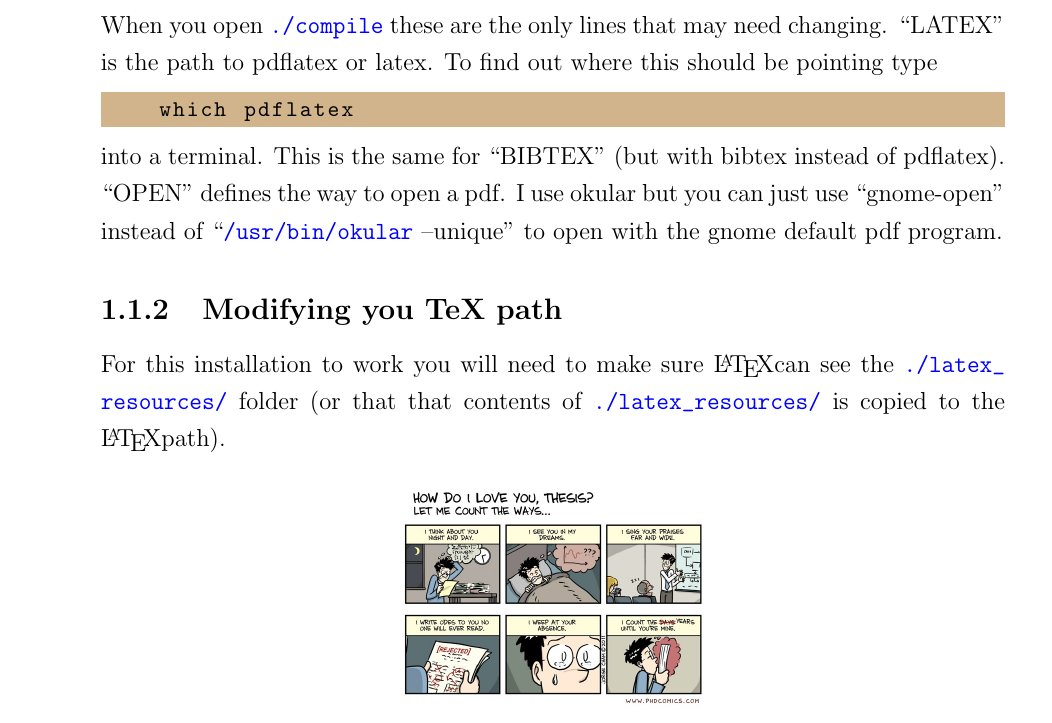
\includegraphics[width=\textwidth]{./figures/phd_comics_example.jpg}
    \\(a)
    \end{center}
    \end{minipage}
    \begin{minipage}{.49\textwidth}
    \begin{center}
    
\includegraphics[width=\textwidth]{./footers/1.jpg}
    \\(b)
    \end{center}
    \end{minipage}
    \end{center}
    \caption[Short title for the list of figures]{Example side by side figure (a) The cartoon footer in the page (b) the jpg file in the \protect\url{./footers} folder. \label{ch1_figure_example_of_side_by_side}}
    \end{figure}

    \vspace{1cm}
    \noindent {\bf \textcolor{red}{NOTE: To turn off the cartoons (enabled by default) just comment out these lines in \url{./main.tex}.}}

    \begin{lstlisting}[style=base]

    @\fancyfoot@[C]{@\includegraphics@[@height@=4cm]
                   {./footers/\arabic{page}.jpg}}

    @\setlength@{@\textheight@}{22.5cm}

    \end{lstlisting}

%------------------------------------------------------------------------------------------------
\subsection{Indexing}
    \label{ch1_section_using_indexing}
%------------------------------------------------------------------------------------------------
    
    There are multiple ways to use the indexing. I use two commands to save on space.

    % This is just how I show code
    \begin{lstlisting}[style=base]
    @\define@{key}
    \end{lstlisting}

    displays the word in the text and adds it to the index. Note that keys are case sensitive and thus will appear multiple times in the index (define also auto capitalises index words so normally I just use the lowercase in the text)

    % This is just how I show code
    \begin{lstlisting}[style=base]
    @\defineas@{word}{key}
    \end{lstlisting}

    displays `word' in the text and adds a different word to the key. An example of when this may be useful is the case where you need a capital word in the text or a word such as `\defineas{photometric}{photometry}', where you only wish to have `\define{photometry}' in the index.

    \begin{lstlisting}[style=base]
    @\index@{key}
    \end{lstlisting}

    puts the key in the index. This requires you to put the word in the text separately.

    Examples of the use are below: 

    \begin{lstlisting}[style=base]
    The @\define@{star} was found by using the 
    @\defineas@{photometric}{photometry} bands, 
    this was useful to judge contamination 
    @\index@{contamination}.
    \end{lstlisting}

    This adds the words `\define{star}', `\define{photometry}' and `\define{contamination}' to the index (with a page reference to this page).

%------------------------------------------------------------------------------------------------
\subsection{Using the glossary}
    \label{ch1_section_using_glossary}
%------------------------------------------------------------------------------------------------

    I use a glossary to define terms such as \acro{2MASS}, \acro{WISE}, \acro{NIR} or \acro{SNR}.
    These words will only appear in the glossary when one of the following commands is used:

    % This is just how I show code
    \begin{lstlisting}[style=base]
    @\acro@{key}
    \end{lstlisting}

    displays the word in the text, and adds the key to the glossary and the index.

    \begin{lstlisting}[style=base]
    @\useglosentry@{key}
    \end{lstlisting} 

    adds the key only to the glossary only.


%------------------------------------------------------------------------------------------------
\subsection{Using acknowledgement citations}
    \label{ch1_section_using_acknowledgement_citations}
%------------------------------------------------------------------------------------------------

    This can be used in any \LaTeX \, document, basically reduces acknowledgements down in to citing the correct survey/telescope or word (acknowledgement terms are stored in \url{./preamble/acknowledgement_refs.tex})

    The can then be used anywhere (\ie at the end of a chapter) using the following command: 

    % This is just how I show code
    \begin{lstlisting}[style=base]
    @\acknowledge@{key}
    \end{lstlisting}

    an example of this is as follows:

    \begin{lstlisting}[style=base]
    @\acknowledge@{2MASS}
    @\acknowledge@{WISE}
    \end{lstlisting}

    And would produce the following text: \\

    \acknowledge{2MASS}

    \acknowledge{WISE}

    Note you can change the word `thesis' for all acknowledgements at the top of the \url{./preamble/acknowledgement_refs.tex} file.

    \subsubsection{Adding new acknowledgements}

    New acknowledgements are set up similar to bibtex files. In \url{./preamble/acknowledgement_refs.tex} keys are set up as follows:

    \begin{lstlisting}[style=base]
    @\pgfkeys@{/APLpy/.code = {This @\acknowledgetype@ made use of 
                               APLpy, an open-source plotting 
                               package for Python hosted at 
                               \url{http://aplpy.github.com}.}}
    \end{lstlisting}

    \noindent where
    \begin{lstlisting}[style=base]
    @\acknowledgetype@
    \end{lstlisting}

    \noindent is set near the start of \url{./preamble/acknowledgement_refs.tex}

    \begin{lstlisting}[style=base]
    \newcommand{\acknowledgetype}{@thesis@\,\,}
    \end{lstlisting}

    \noindent editing the text in red in the above will change all acknowledgements to use this instead of thesis (see above).



%------------------------------------------------------------------------------------------------
\subsection{Referencing Figures, Tables and Sections}
    \label{ch1_section_ref_fig_tab_sec}
%------------------------------------------------------------------------------------------------

    These are short cuts to writing ``Figure X'', ``Table Y'', ``Section Z'' and are edited in the \url{./preamble/newcommands.tex}.

    These are defined for a figure:

    % This is just how I show code
    \begin{lstlisting}[style=base]
    @\reffig@{reference}
    \end{lstlisting}

    \noindent the above is an alias of:

    \begin{lstlisting}[style=base]
    Figure @\ref@{reference}
    \end{lstlisting}

    A table:

    \begin{lstlisting}[style=base]
    @\reftab@{reference}
    \end{lstlisting}

    \noindent the above is an alias of:

    \begin{lstlisting}[style=base]
    Table @\ref@{reference}
    \end{lstlisting}

    And a section:

    \begin{lstlisting}[style=base]
    @\refsec@{reference}
    \end{lstlisting}

    \noindent the above is an alias of:

    \begin{lstlisting}[style=base]
    Section @\ref@{reference}
    \end{lstlisting}
    
    \noindent These aliases can be changed in \url{./preamble/newcommands.tex}:

    \begin{lstlisting}[style=base]
    %referencing sections, figures, tables, equations
    \newcommand{\reffig}[1]{@Figure@ \ref{#1}}
    \newcommand{\reftab}[1]{@Table@ \ref{#1}}
    \newcommand{\refequ}[1]{@Equation@ \ref{#1}}
    \newcommand{\refsec}[1]{@Section@ \ref{#1}}
    \end{lstlisting}

    \noindent \ie replacing Figure with Fig. will change every instance of reffig.

    An example of each is shown below:

    \begin{lstlisting}[style=base]
    \reffig{ch1_figure_1} shows x against y 
    (from \refsec{ch1_section_2}) and 
    is also shown in \reftab{ch1_table_3}.
    \end{lstlisting}

    This would give the following text:

    Figure 1 shows x against y (from Section 1.2) and is also shown in Table 3.